\section{Background} \label{sec:background}
  \subsection{Rowhammer Attack} \label{subsec:rowhammer-attack}
    Rowhammer is a main memory attack triggered by a software-induced hardware 
    fault to flip bits soley with increased pressure caused by frequent reads 
    to selected memory rows.
    \\
    From a technical perspective, the Rowhammer workflow begins with the attacker 
    placing data in memory through arbitrary memory allocation. Subsequently, 
    specific \gls{dram} rows are filtered and addressed together in a targeted manner 
    by reading them at a very high frequency, a process commonly referred to as 
    “hammering”. During this process, the cache is consistently bypassed using 
    eviction strategies or explicit flush instructions. The hammering technique 
    is crucial, as it determines which victim row is targeted, how many aggressor 
    rows are involved, and their relative distances to the victim rows. These 
    factors decisively influence the frequency of observable bit flips, even in 
    the presence of mitigation mechanisms.
    \\
    As a consequence of continuous hammering, adjacent \gls{dram} rows are exposed to 
    repeated gate-induced drain and subthreshold leakage~\cite{paperFlippingBits, paperRHinDRAM}. This leads to 
    sufficient charge loss~\cite{paperTriggeringRHHardwareFault} and electrical disturbance~\cite{paperRowhammerOnSteroids}, ultimately 
    causing memory cells to flip from 0 to 1 or vice versa.

  \subsection{Memory Addressing} \label{subsec:memory-addressing}
    To understand how Rowhammer attacks are designed, it is first necessary to 
    examine how software running on a system is able to access hardware components 
    such as \gls{dram}. This interaction fundamentally relies on the use of memory 
    addresses.
    \\
    Memory addresses are required because they uniquely identify and locate data, 
    allowing systems to store and later retrieve the same information reliably, 
    independent of its physical realization. In this context, 
    two types of memory addresses can be distinguished.
    \\
    Virtual addresses are generated and used by processes and define a per-process 
    virtual address space that is independent of the underlying physical 
    memory~\cite{webVirtualAddress}. The size of this virtual address space depends on the system 
    architecture, such as the \gls{cpu} register width, and may exceed the amount of 
    available physical \gls{ram}~\cite{blogVirtualMemory}. In contrast, physical addresses refer to actual 
    locations in main memory and constitute the system-wide physical address 
    space corresponding to the installed \gls{ram}~\cite{blogVirtToPhys}. Physical addresses are globally 
    unique within the system~\cite{blogVirtualMemory}.
    \\
    Processors employ virtual memory systems in which virtual addresses are 
    translated into physical addresses~\cite{toolRPI3}. These memory translations, also 
    referred to as mappings, are achieved by the system resolving the physical memory 
    address corresponding to a given virtual address~\cite{blogVirtToPhys}. Page tables play a 
    central role in defining and managing these virtual-to-physical address mappings.
    \\
    A page table consists of numerous \gls{pte}s~\cite{blogVirtToPhys}. Page tables 
    store the mapping between virtual and physical addresses, including associated 
    attributes, and these entries are used by the \gls{tlb} 
    as a fast cache to accelerate address translation~\cite{blogVirtualMemory, docPageTables}.
    \\
    The kernel provides an interface exposed via \texttt{/proc/pagemap}, which returns a 
    64-bit value containing page table-related information. This information 
    includes whether and how a page is located in \gls{ram} or swap, as well as which 
    physical memory area it maps to~\cite{docExaminingPageTables}.
    \\
    Page tables are typically managed by the \gls{mmu}~\cite{webVirtualMemoryTranslation, blogVirtToPhys}. 
    The \gls{mmu} is a hardware component responsible for translating virtual addresses 
    into physical addresses~\cite{blogVirtToPhys}. When the \gls{cpu} attempts to access a memory location, 
    it supplies a virtual address to the \gls{mmu}, which then verifies if a corresponding 
    translation already exists in the \gls{tlb}~\cite{docPageTables}.
    \\
    On a memory access, the \gls{cpu} supplies a virtual address to the \gls{mmu}, which first 
    consults the \gls{tlb}, a cache of recent address translations integrated into the 
    \gls{mmu}~\cite{webVirtualMemoryTranslation}, to quickly resolve the corresponding physical address~\cite{docPageTables}. By avoiding 
    frequent page table lookups in main memory, the \gls{tlb} significantly reduces the 
    latency of address translation~\cite{webVirtualMemoryTranslation, blogVirtToPhys}.
    \\
    Functionally, the virtual address is first divided into a virtual page number 
    and a page offset~\cite{blogVirtToPhys}. The page offset is passed through unchanged, as it does 
    not require translation. The virtual page number is then looked up in the \gls{tlb} by 
    searching for a matching tag. In the case of a \gls{tlb} hit, the physical address is 
    returned immediately. In the case of a \gls{tlb} miss, the \gls{mmu} accesses main memory 
    to locate the corresponding page frame. If the entry is found, the translation 
    is completed and cached in the \gls{tlb}. If no entry exists, the system may need to 
    retrieve the page from storage, which represents the worst-case 
    scenario.

  \subsection{Timing Measurement} \label{subsec:timing-measurement}
    Timing serves as the basic for identifying \gls{dram} accesses and is an 
    essential part of executing or reverse engineering rowhammer attacks, particularly 
    when adapting such attacks to ARM-based systems for the development of Proof of Concept (PoC)
    implementations. On x86 architectures, high-resolution timestamps can be obtained 
    in an unprivileged context using the \gls{rdtsc} instruction. The \gls{rdtsc} 
    instruction provides an unprivileged mechanism for acquiring sub-nanosecond timing information.
    It functions as a fine-grained timer by returning a high-resolution count of CPU clock cycles.
    In contrast, ARM architectures, specifically ARMv7-A and ARMv8-A, do not offer a 
    direct counterpart to the \gls{rdtsc} instruction. Instead, high-resolution timing on 
    these systems can be acquired via the \gls{pmu} cycle counter, 
    referred to as \texttt{PMCCNTR}, which counts processor cycles. While these measurements enable 
    fast and precise timing, access to the performance counters is generally restricted to 
    kernel space by default~\cite{thesisCacheAttacksandRH, thesisDRAMA}.
    \\
    The \texttt{PMCCNTR\_EL0} register holds the value of the processor cycle counter,
    monitoring the number of processor clock cycles. It is a 64-bit register 
    integrated within the \gls{pmu} block. Architecturally, the external register 
    \texttt{PMCCNTR\_EL0} bits \texttt{[63:0]} are mapped to the AArch64 system 
    register. The increment behavior of the cycle counter 
    is determined by the configuration of the \texttt{PMCR\_EL0 {LC, D}} control bits, 
    allowing the counter to advance either on every processor clock cycle or on 
    every 64th processor clock cycle. Following a warm reset, \texttt{PMCCNTR\_EL0} is 
    initialized to an architecturally undefined value~\cite{paperPMCCNTREL0}.

  \subsection{Cache Organization} \label{subsec:cache-organization}
      %% Direct-mapped Caches
      In a direct-mapped cache, each main memory entry is mapped to exactly one cache location. As a 
      consequence, multiple distinct memory addresses can also map to the same cache location~\cite{thesisCacheAttacksandRH}.
      \\
      An illustrative example is shown in \hyperref[fig:direct-mapped-cache]{Figure~\ref{fig:direct-mapped-cache}}, which depicts a cache with a total size of 4~KB, 
      consisting of 128 cache locations and a cache line size of 64~bytes. In this configuration, an address 
      is divided into three fields: 6 bits for the block offset, 7 bits for the index, and 19 bits for the 
      tag.
      \begin{figure}[htbp]
          \centering
          \frame{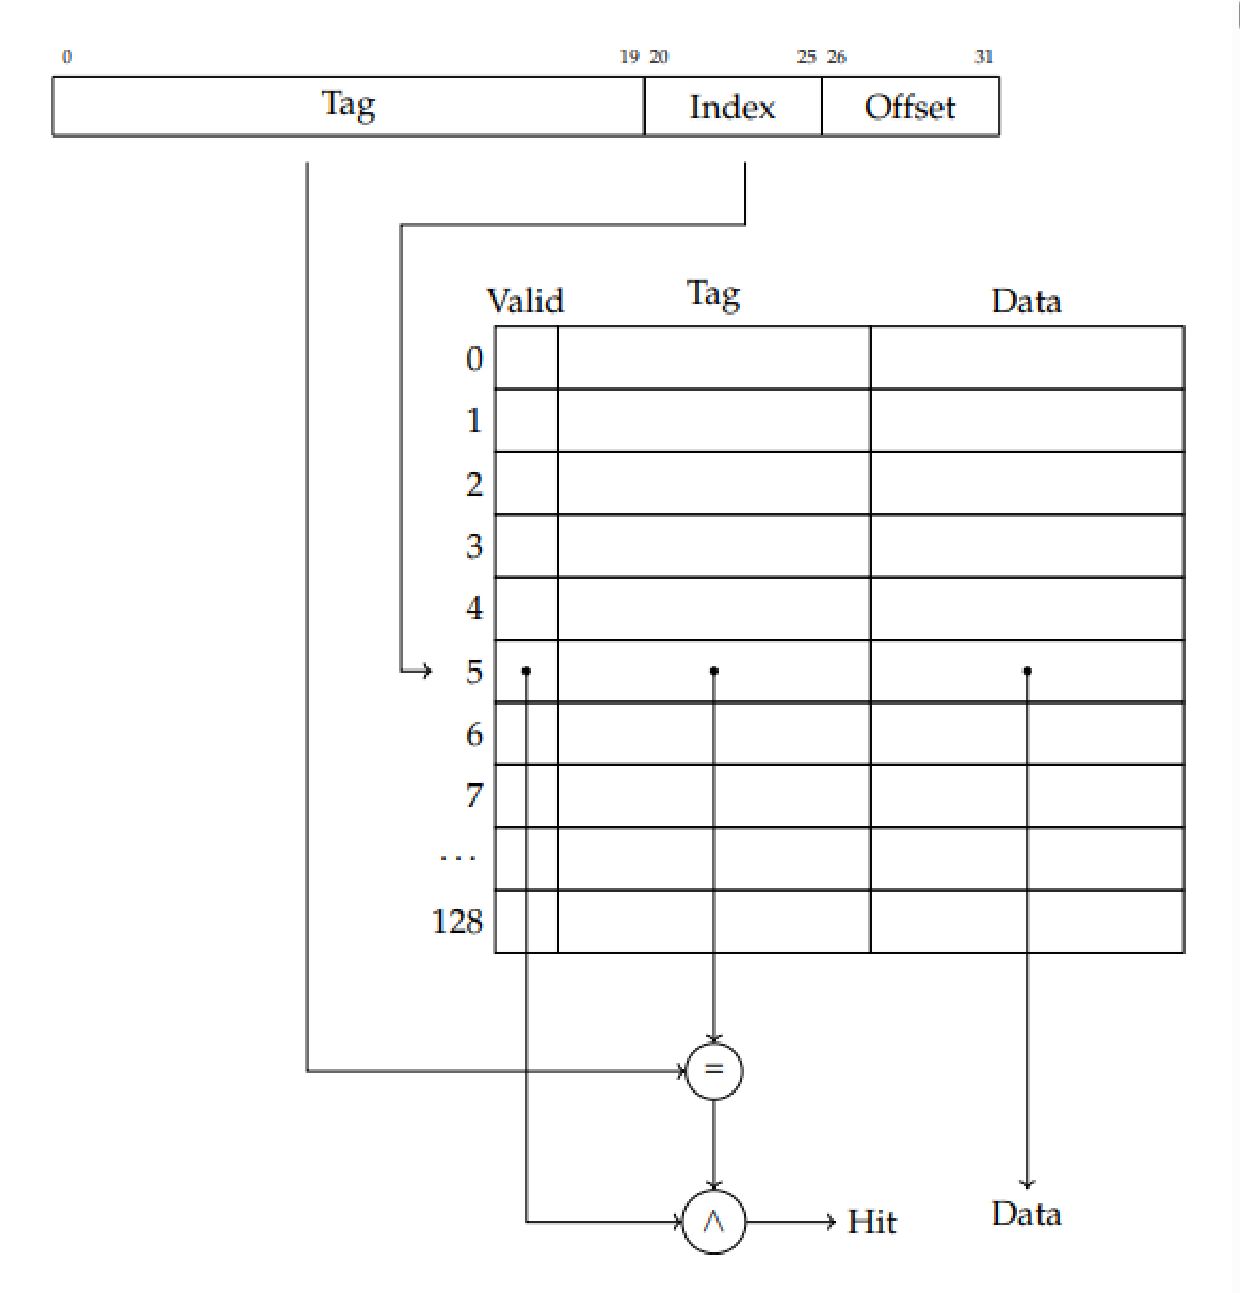
\includegraphics[width=\linewidth]{img/direct-mapped-cache.pdf}}
          \caption{Direct-mapped cache~\cite{thesisCacheAttacksandRH}}
          \label{fig:direct-mapped-cache}
      \end{figure}
      To determine whether a specific address is present in the cache, the index bits of the address are 
      first identified, and the associated cache line's stored tag is then compared with the address's tag.
      If the tags match and the valid bit is set, a cache hit occurs, and the block offset is used to select 
      the relevant word from the cache line. If the tags do not match or the valid bit is not set, indicating 
      that the cache entry does not contain valid data, a cache miss occurs, and the cache line is replaced 
      with data fetched from the requested memory address.

      %% Set-Associative Caches
      If the replacement policy is allowed to choose any entry in the cache to hold a the data, the 
      cache is referred to as fully associative~\cite{thesisCacheAttacksandRH}. Modern processors, however, typically employ 
      set-associative caches, which organize cache lines into multiple sets~\cite{thesisCacheAttacksandRH}. In an N-way set-associative 
      cache, each memory block can be placed in any one of N cache lines within a specific set.
      \\
      Each memory address maps to exactly one cache set, and addresses that map to the same set are called 
      congruent addresses, as illustrated in \hyperref[fig:n-way-associative-cache]{Figure~\ref{fig:n-way-associative-cache}}. 
      When all cache lines of a set are occupied and a new block needs to be loaded, the cache replacement 
      policy determines which existing cache line is evicted in order to accommodate the new data~\cite{thesisCacheAttacksandRH}.

      \begin{figure}[htbp]
          \centering
          \frame{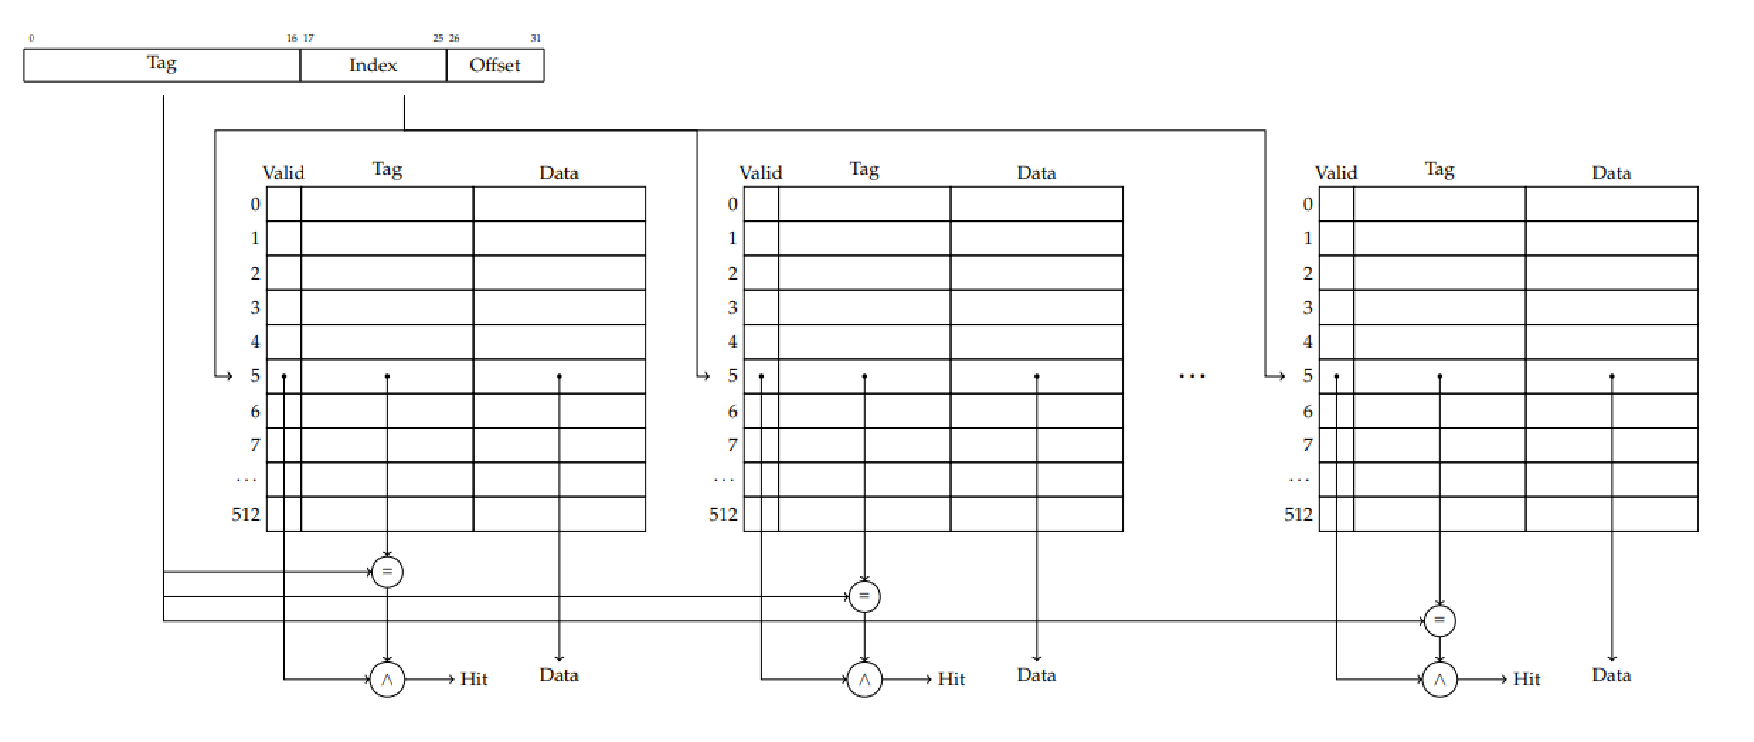
\includegraphics[width=\linewidth]{img/n-way-associative-cache.pdf}}
          \caption{N-way associative cache~\cite{thesisCacheAttacksandRH}}
          \label{fig:n-way-associative-cache}
      \end{figure}

      \begin{table}[h!]
          \centering
          \caption{RPi4 Cache: \texttt{lscpu {-}{-}cache}}
          \label{tab:rpi4-cache}
          \resizebox{\textwidth}{!}{%
              \begin{tabular}{lrrrrrrr}
                  \hline
                  NAME & ONE-SIZE & ALL-SIZE & WAYS & TYPE & LEVEL & SETS & COHERENCY-SIZE \\
                  \hline
                  L1d & 32K  & 128K  & 2  & Data        & 1 & 256  & 64 \\
                  L1i & 48K  & 192K  & 3  & Instruction & 1 & 256  & 64 \\
                  L2  & 1M   & 1M    & 16 & Unified     & 2 & 1024 & 64 \\
                  \hline
              \end{tabular}%
          }
      \end{table}
      \begin{table}[h!]
          \centering
          \caption{RPi5 Cache: \texttt{lscpu {-}{-}cache}}
          \label{tab:rpi5-cache}
          \resizebox{\textwidth}{!}{%
              \begin{tabular}{lrrrrrrr}
                  \hline
                  NAME & ONE-SIZE & ALL-SIZE & WAYS & TYPE & LEVEL & SETS & COHERENCY-SIZE \\
                  \hline
                  L1d & 64K  & 256K  & 4  & Data        & 1 & 256  & 64 \\
                  L1i & 64K  & 256K  & 4  & Instruction & 1 & 256  & 64 \\
                  L2  & 512K & 2M    & 8  & Unified     & 2 & 1024 & 64 \\
                  L3  & 2M   & 2M    & 16 & Unified     & 3 & 2048 & 64 \\
                  \hline
              \end{tabular}%
          }
      \end{table}
      \hyperref[tab:rpi4-cache]{Tables \ref{tab:rpi4-cache}} and \ref{tab:rpi5-cache} summarize the cache configurations of the Raspberry 
      Pi 4 and Raspberry Pi 5, respectively. These tables provide 
      an overview of cache sizes, associativity, cache levels, and the number of cache sets for the different 
      cache hierarchies present on both platforms.
      
      The number of cache sets is determined by the cache size, the cache line size, and the set associativity. 
      This relationship can be expressed as
      \[
      2^{\text{Index}} = \frac{\text{Cache Size}}{\text{Line Size} \times \text{Set associativity}}
      \]
      Applying this formula to the L2 cache of the Raspberry Pi 4 results in
      \[
      \text{Number of sets} = \frac{1024 \times 1024}{64 \times 16} = 1024 = 2^{10}
      \]
      Similarly, for the L2 cache of the Raspberry Pi 5, the number of cache sets is given by
      \[
      \text{Number of sets} = \frac{512 \times 1024}{64 \times 8} = 1024 = 2^{10}
      \]
      These calculations show that, despite differences in cache size and associativity, both systems employ 
      the same number of cache sets at the L2 cache level.
      \\

      %% Virtual and Physical Tags and Indexes
      \noindent
      \gls{cpu} caches can be indexed and tagged using either virtual or physical addresses. When virtual 
      addresses are used, it is possible for the same physical address to be cached in multiple cache lines, 
      which can negatively affect performance. Cache lines are uniquely identified by a tag, which may 
      be derived from either the virtual or the physical address~\cite{thesisCacheAttacksandRH}.
      \\
      In \textbf{\gls{vivt}} caches, both the index and the tag are derived from the 
      virtual address. Such caches are generally faster because no address translation is required before 
      lookup; however, the virtual tag is not unique, and shared memory may appear multiple times in the cache.
      \\
      \textbf{\gls{pipt}} caches use the physical address for both index and tag. 
      This approach avoids duplication of shared memory in the cache, but it is slower because address 
      translation via the \gls{tlb} is required before cache access.
      \\
      \textbf{\gls{pivt}} caches use the physical address for indexing and the virtual 
      address for tagging. This design provides no practical benefit, as it still requires address translation 
      while retaining the disadvantage of non-unique virtual tags, allowing shared memory to be duplicated.
      \\
      \textbf{\gls{vipt}} caches use the virtual address for indexing and the physical 
      address for tagging. This approach offers lower latency than \gls{pipt} caches because index lookup can proceed 
      in parallel with \gls{tlb} translation, although tag comparison must still wait for the physical address.
      \\
      On the Raspberry Pi 4, the L1 instruction cache, L1 data cache, and L2 cache behave as \gls{pipt} caches~\cite{webRPi4Hardware, docCortexA72}. 
      On the Raspberry Pi 5, the L1 instruction and L1 data caches are \gls{vipt}, but they behave effectively as \gls{pipt}
      4-way set-associative caches~\cite{docCortexA76}.